% Prof. Dr. Ausberto S. Castro Vera
% UENF - CCT - LCMAT - Curso de Ci\^{e}ncia da Computa\c{c}\~{a}o
% Campos, RJ,  2023
% Disciplina: Paradigmas de Linguagens de Programa\c{c}\~{a}o
%


\chapter{Ferramentas existentes e utilizadas}

Neste capítulo iremos aprender um pouco sobre as ferramentas utilizadas nesse livro. Entender desde o motivo da utilização de cada uma até um panorama geral de como elas funcionam. Vamos aprender um pouco mais sobre toda a ambientação do R e o que precisamos instalar e preparar para partirmos à prática.



    \section{Interpretador R}
    \cite{Davies2016} Diz que a R é uma linguagem interpretada, ou seja, o programa é traduzido e executado linha por linha, sem a necessidade de uma compilação completa, o que facilita a visibilidade das operações, coisa que falaremos mais para frente. O que nos importa é que precisaremos do software para a interpretação de cada linha, encontraremos o interpretador R para baixar e instalar no site oficial: \url{https://www.r-project.org}, O site oferece uma ampla gama de informações sobre a linguagem e o software, incluindo sua história, membros da comunidade e um blog com atualizações constantes.No site oficial, encontraremos o CRAN (Comprehensive R Archive Network), onde estão as versões atualizadas para download do software e suas documentações. Atualmente estando na versão 4.3.0.
    \begin{figure}[H]
    	\centering
    	\caption{O CRAN.}
    	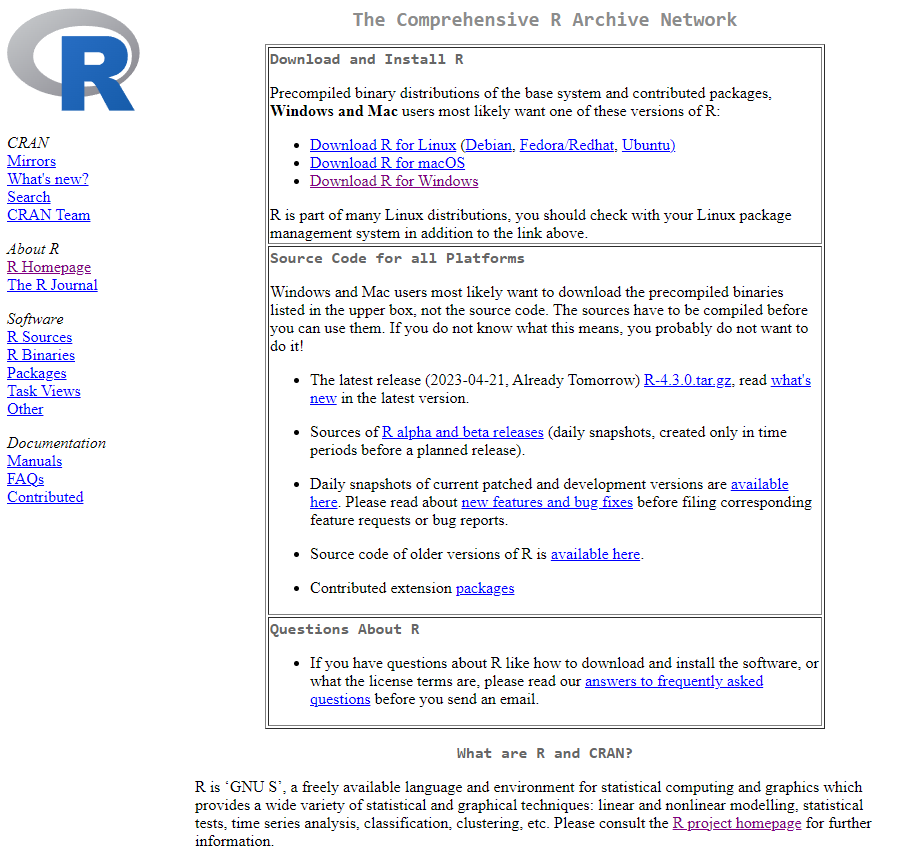
\includegraphics[width=1.0\linewidth]{Prints/screenshot026}
    	\label{fig:screenshot026}
    	{\tiny \sf Fonte:\url{https://https://vps.fmvz.usp.br/CRAN/} }
    \end{figure}
    
	\section{Editor R GUI}
	Assim que instalamos o software R com o interpretador, também recebemos o editor R GUI (Graphical User Interface), que nada mais é do que uma simples interface de utilização básica do aplicativo:\begin{figure}[H]
		\centering
		\caption{O editor GUI}
		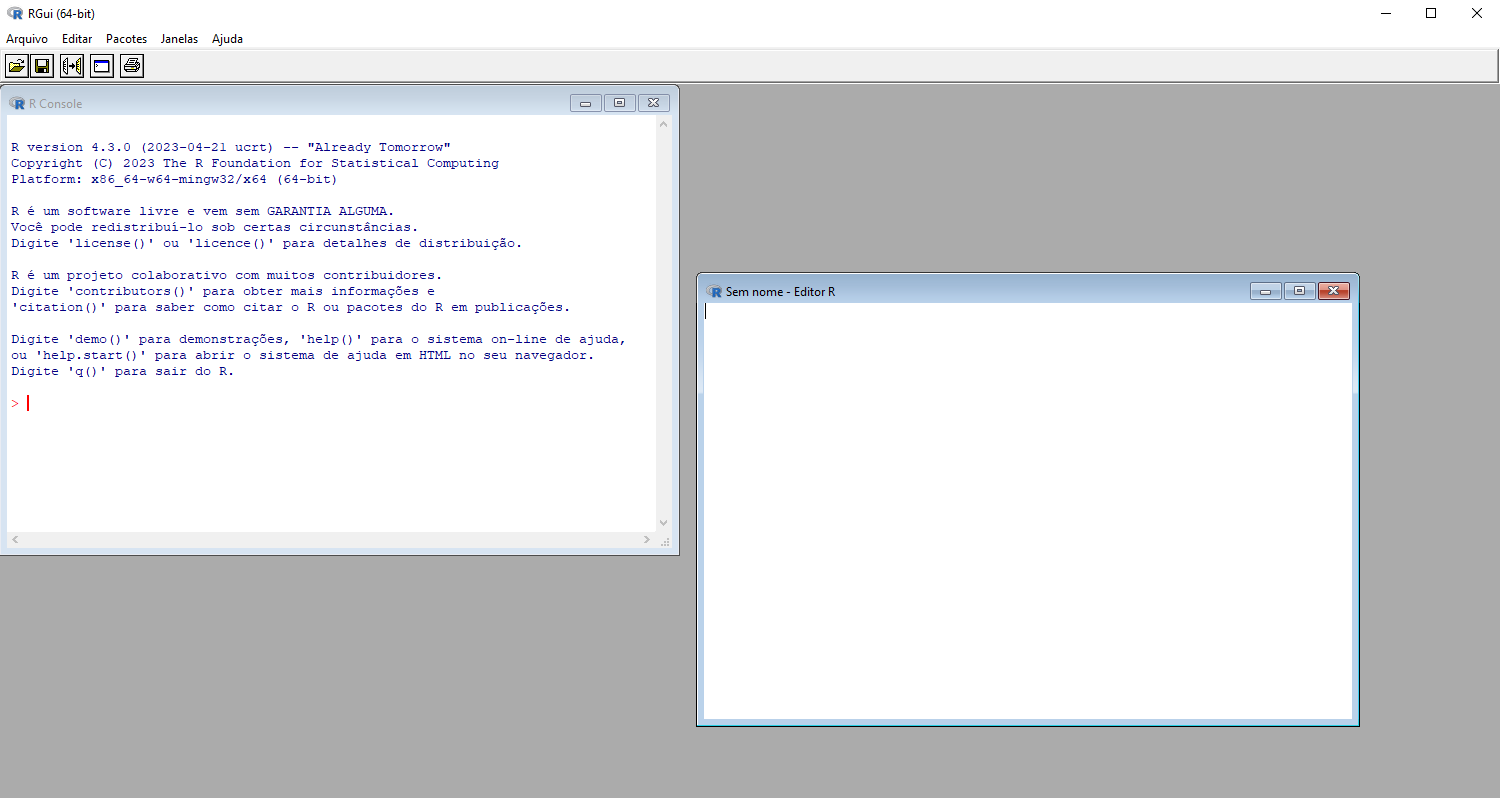
\includegraphics[width=1.0\linewidth]{Prints/screenshot027}
		\label{fig:screenshot027}
		{\tiny \sf Fonte: O autor deste trabalho }
	\end{figure}
	Como podemos ver, é a aplicação do R em sua forma mais básica. Temos uma página com o console, onde mostra cada linha sendo interpretada e executada, e ao lado o editor, onde os códigos podem ser escritos e editados. Além disso, apenas algumas opções de edição do ambiente, e principalmente a aba de instalação de pacotes.\par
	Por conta de ser simples até demais, utilizaremos outro editor, que é um IDE. Veremos mais à seguir.
    \section{Ambientes de Programa\c{c}\~{a}o IDE Rstudio}
    
    Um IDE (Integrated Development Environment) é um programa para o auxilio dos desenvolvedores, que reúne em apenas um programa diversas ferramentas que podem ser necessárias para a produtividade de um código. Um programa pode ser escrito em um editor de texto qualquer, no entanto, é preferível a utilização de IDEs para maior desempenho.\par 
    Nesse caso, utilizaremos o Rstudio, um dos mais importantes IDEs para a linguagem R. Citando diretamente do site \url{https://posit.co/download/rstudio-desktop/}, Rstudio é um kit de ferramentas feito pra nos ajudar a sermos mais produtivos com R e Python. Levando essa definição em conta, vamos ver em que consiste o Rstudio: \begin{figure}[H]
    	\centering
    	\caption{Rstudio}
    	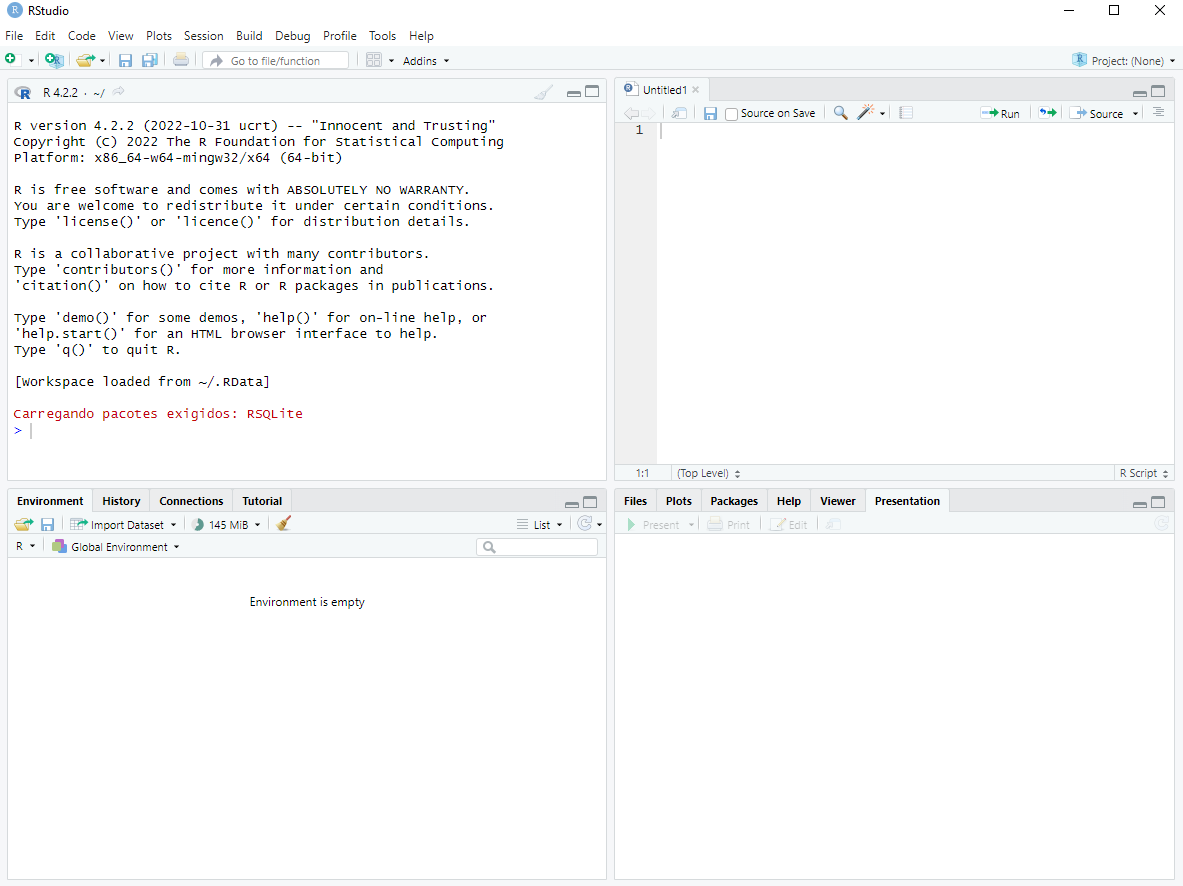
\includegraphics[width=1.0\linewidth]{Prints/screenshot028}
    	\label{fig:screenshot028}
    	{\tiny \sf Fonte: O autor deste trabalho }
    \end{figure}

	O ambiente é dividido em quatro painéis, que podem ser minimizados e maximizados como o usuário quiser. No exemplo acima pode-se ver o console R(Superior Esquerdo), o editor de texto R (Superior Direito), a aba de arquivos (Inferior Direito) e a aba com o ambiente das variáveis (Inferior Esquerdo)\par
	A configuração desses painéis pode ser alterada a partir da aba de configuração geral do aplicativo:\begin{figure}[H]
		\centering
		\caption{Edição dos painéis}
		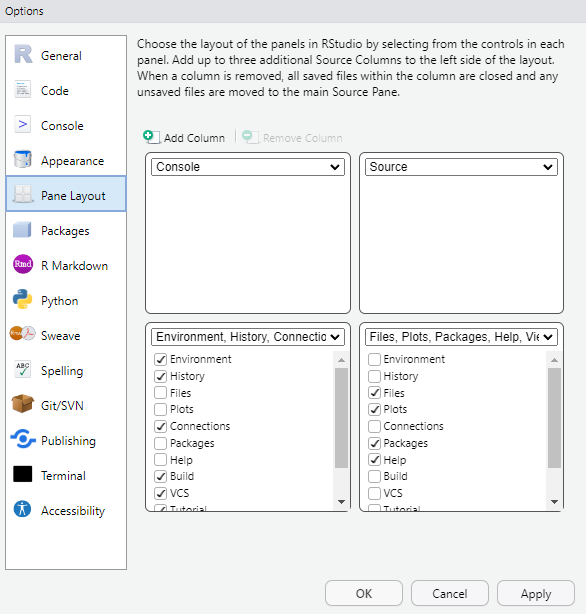
\includegraphics[width=1.0\linewidth]{Prints/screenshot029}
		\label{fig:screenshot029}
		{\tiny \sf Fonte: O autor deste trabalho }
	\end{figure}\par 

		Essa é uma visão geral do que é encontrado nesse ambiente, mas como o site afirma, é um kit de ferramentas que possui diversas outras utilidades.\par
		A download se encontra no site: \url{https://posit.co/download/rstudio-desktop/} sendo a versão 4.1.2.
	
	
    